\let\negmedspace\undefined
\let\negthickspace\undefined
\documentclass[journal]{IEEEtran}
\usepackage[a5paper, margin=10mm, onecolumn]{geometry}
%\usepackage{lmodern} % Ensure lmodern is loaded for pdflatex
\usepackage{tfrupee} % Include tfrupee package

\setlength{\headheight}{1cm} % Set the height of the header box
\setlength{\headsep}{0mm}     % Set the distance between the header box and the top of the text

\usepackage{gvv-book}
\usepackage{gvv}
\usepackage{cite}
\usepackage{amsmath,amssymb,amsfonts,amsthm}
\usepackage{algorithmic}
\usepackage{graphicx}
\usepackage{textcomp}
\usepackage{xcolor}
\usepackage{txfonts}
\usepackage{listings}
\usepackage{enumitem}
\usepackage{mathtools}
\usepackage{gensymb}
\usepackage{comment}
\usepackage[breaklinks=true]{hyperref}
\usepackage{tkz-euclide} 
\usepackage{listings}
% \usepackage{gvv}                                        
\def\inputGnumericTable{}                                 
\usepackage[latin1]{inputenc}                                
\usepackage{color}                                            
\usepackage{array}                                            
\usepackage{longtable}                                       
\usepackage{calc}                                             
\usepackage{multirow}                                         
\usepackage{hhline}                                           
\usepackage{ifthen}                                           
\usepackage{lscape}
\begin{document}

\bibliographystyle{IEEEtran}
\vspace{3cm}

\title{1.4.9.9}
\author{EE24BTECH11047 - Niketh Prakash Achanta
}
% \maketitle
% \newpage
% \bigskip
{\let\newpage\relax\maketitle}

\renewcommand{\thefigure}{\theenumi}
\renewcommand{\thetable}{\theenumi}
\setlength{\intextsep}{10pt} % Space between text and floats


\renewcommand{\thetable}{\theenumi}


\textbf{Question}: \\
Find the coordinates of the points of trisection \brak{i.e.\ points\ dividing\ to\ three\ equal\ parts} of the line segment joining the points $\vec{A\brak{2,-2}\ \text{and}\ B\brak{-7,4}}$.
\\
\textbf{Solution: }
\begin{table}[h!]    
  \centering
  \begin{tabular}[12pt]{ |c| c|}
    \hline
    \textbf{Variable} & \textbf{Description}\\ 
    \hline
    $A$ & One end of line segment \\
    \hline 
    $B$ & Other end of line segment \\
    \hline
    $P_1$ & First point of trisection \\
    \hline
    $P_2$ & Second point of trisection \\
    \hline
    $m$ & Ratio in which $P_1$ divides AB \\
    \hline
    $n$ & Ratio in which $P_2$ divides AB \\
    \hline
    \end{tabular}

  \caption{Variables Used}
  \label{tab1.1.4.9.9.1}
\end{table}
\\
Using the section formula:
\begin{align}
	\vec{C}=\brak{\frac{\vec{B}+m\vec{A}}{1+m}} \label{eq1.1.4.9.9.1}
\end{align}
\begin{align}
	\vec{P1 \text{or} P2}= \myvec{\frac{-7+2m}{1+m} \\ \frac{4-2m}{1+m}} \label{eq1.1.4.9.9.2}
\end{align}
$\vec{P1}$ divides AB in the ratio $1:2$, so 
\begin{align}
	m=\frac{1}{2}
\end{align}
Plugging this value in \ref{eq1.1.4.9.9.2}, we get
\begin{align}
	\vec{P1} = \myvec{-1 \\ 0}
\end{align}
Similarly, in case of $\vec{P2}$,
\begin{align}
	n=2
\end{align}
Again, putting this value in place of $m$ in \ref{eq1.1.4.9.9.2}, we get
\begin{align}
	\vec{P2} = \myvec{-4 \\ 2}
\end{align}
Thus, we have found the points of intersection viz. $\vec{P1} = \myvec{-1 \\ 0}$ and $\vec{P2} = \myvec{-4 \\ 2}$ . 
\begin{figure}[h]
	\centering
	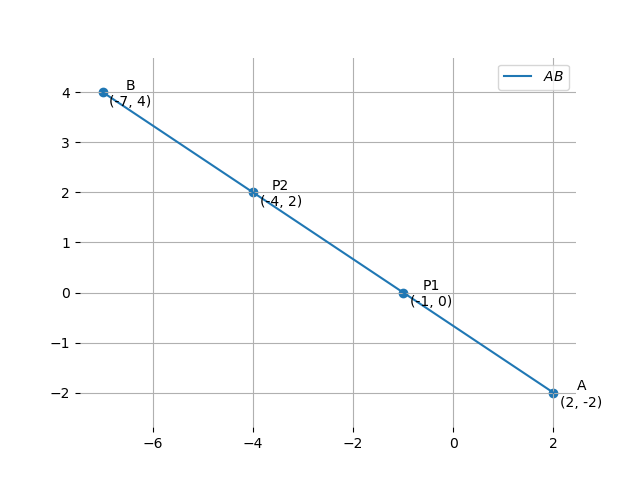
\includegraphics[width=0.7\linewidth]{figs/fig1.png}
	\caption{}
	\label{graph}
\end{figure}
\end{document}




